\documentclass[serif,9pt]{beamer}
\usetheme{tree}

\usepackage[latin1]{inputenc}
\usepackage[spanish]{babel}

% Images
\usepackage{graphicx}
\usepackage{subfigure} % subfiguras
\usepackage{caption}
\usepackage{float}
\captionsetup[table]{labelformat=empty}
\captionsetup[figure]{labelformat=empty}

\usepackage{animate}

\usepackage{amsmath}

\usepackage{xcolor}
\definecolor{gray}{rgb}{0.5,0.5,0.5}
\usepackage{hyperref}
            
\AtBeginSection[]
{
  \begin{frame}<beamer>{Contenido}
    \tableofcontents[currentsection]
  \end{frame}
}

\begin{document}
\setbeamertemplate{navigation symbols}{}

\title{BitTorrent}  
\author{David Cabezas Berrido y Patricia C�rdoba Hidalgo}
\date{}

\begin{frame}
\titlepage
\end{frame}

\begin{frame}\frametitle{�ndice}
  \tableofcontents
\end{frame}

\section{Introducci�n}

\begin{frame}\frametitle{Introducci�n}
  \begin{figure}[H]
    \raggedright
    
\includegraphics[width=70mm]{imagenes/bram_cohen}
  \end{figure}
  
  \begin{figure}[H]
    \raggedleft
    
\includegraphics[width=60mm]{imagenes/clientes}
  \end{figure}
\end{frame}

\section{Arquitectura Peer-to-Peer (P2P)}

\begin{frame}\frametitle{Arquitectura Peer-to-Peer (P2P)}
  \begin{figure}[H]
    \centering
    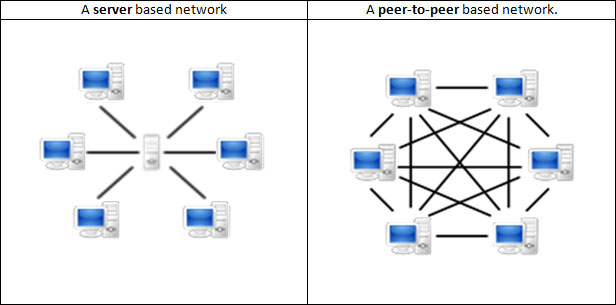
\includegraphics[width=110mm]{imagenes/p2p-networks}
  \end{figure}

\end{frame}

\subsection{Escalabilidad en P2P para distribui�n de archivos}

\begin{frame}\frametitle{Escalabilidad en P2P para distribui�n de archivos}
  Queremos compartir un archivo. Sea:
  \begin{itemize}
  \item $N$ - n� clientes 
  \item $F$ - tama�o del archivo (bytes)
  \item $u_s$ - velocidad de subida del servidor (bytes/s)
  \item $u_i$ - velocidad de subida del cliente i-�simo (bytes/s)
  \end{itemize}

  \vspace{5mm}

  Tiempo de distribuci�n en CS es al menos: $\dfrac{NF}{u_s}$ segundos.\\
  \vspace{8mm}
  Tiempo de distribuci�n en P2P es al menos:  $\dfrac{NF}{u_s+\sum\limits_{i=1}^{N}u_i}$ segundos.
\end{frame}

\begin{frame}\frametitle{Ejemplo}
  
Suponiendo $u_i=u \hspace{0.2cm} \forall i$, $\frac{F}{u} = 1 h$ y $u_s = 10u$:
  \begin{figure}[H]
    \centering
    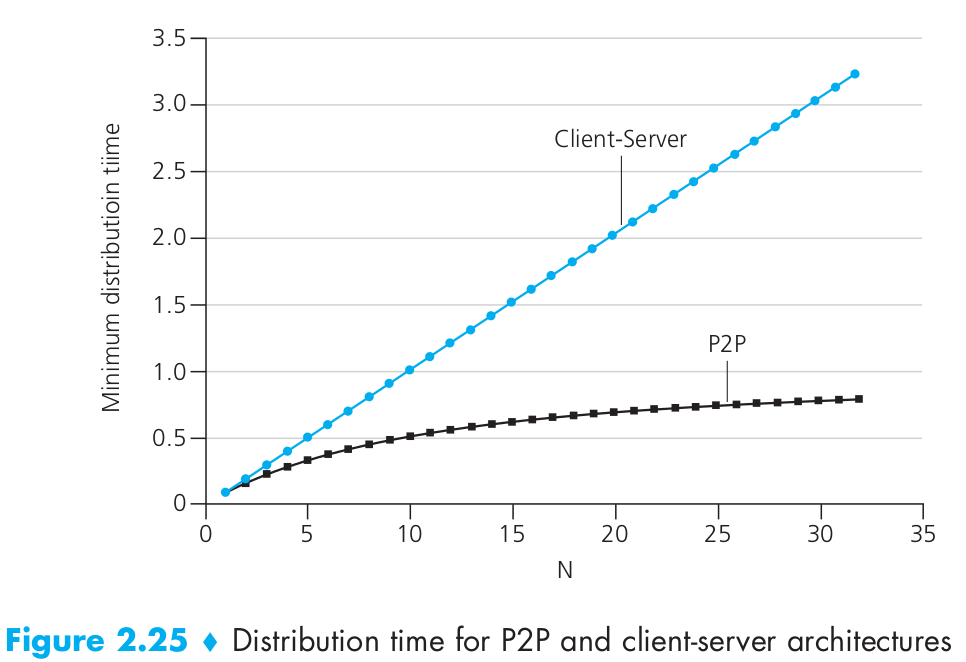
\includegraphics[width=90mm]{imagenes/Escalabilidad}
        \caption{Kurose, Ross 2013 (Cap�tulo 2, p�gina 148)}
  \end{figure}

\end{frame}

\section{El protocolo BitTorrent}

\begin{frame}\frametitle{Mecanismo b�sico}
  \begin{itemize}
  \item Descargar y ejecutar el archivo \texttt{.torrent}.
  \item Unirse al \textit{torrent}.
  \item Comunicarse con el \textit{tracker}.
  \item Establecer comunicaci�n (TCP) con sus ``vecinos''.
  \item Intercambiar \textit{chunks} con ellos.
  \end{itemize}
\end{frame}

\begin{frame}\frametitle{Intercambio de chunks}

  \begin{itemize}
  \item Solicitar lista de chunks a los vecinos.
  \item Solicitar chunks (heur�stica del m�s raro).
  \item Atender solicitudes (``Tit for tat'').
  \item \textit{Optimistic Unchoking}.
  \end{itemize}
  
\end{frame}

% \begin{frame} \frametitle{El protocolo BitTorrent}
% \vspace{-2mm}
%   \begin{figure}[H]
%     \centering
%     \animategraphics[loop,controls,width=75mm]{imagenes/50}{animation/bittorrent-animation-}{0}{9}
%   \end{figure}
% \end{frame}

% Animacion 0
\begin{frame} \frametitle{El protocolo BitTorrent}
\vspace{-2mm}
  \begin{figure}[H]
    \centering
    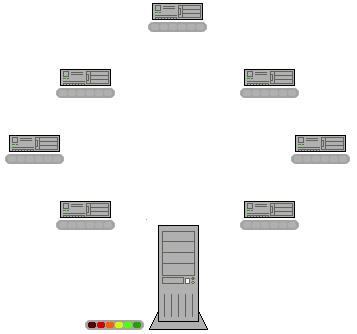
\includegraphics[width=80mm]{imagenes/animation/bittorrent-animation-0}
  \end{figure}
\end{frame}

% Animacion 1
\begin{frame} \frametitle{El protocolo BitTorrent}
\vspace{-2mm}
  \begin{figure}[H]
    \centering
    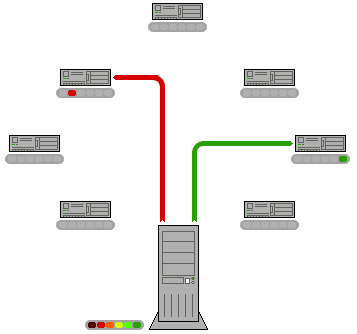
\includegraphics[width=80mm]{imagenes/animation/bittorrent-animation-1}
  \end{figure}
\end{frame}

% Animacion 2
\begin{frame} \frametitle{El protocolo BitTorrent}
\vspace{-2mm}
  \begin{figure}[H]
    \centering
    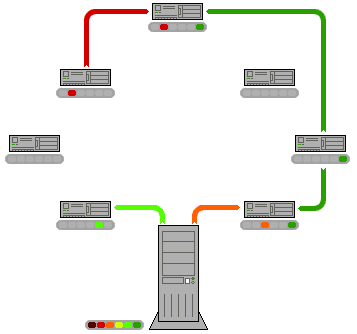
\includegraphics[width=80mm]{imagenes/animation/bittorrent-animation-2}
  \end{figure}
\end{frame}

% Animacion 3
\begin{frame} \frametitle{El protocolo BitTorrent}
\vspace{-2mm}
  \begin{figure}[H]
    \centering
    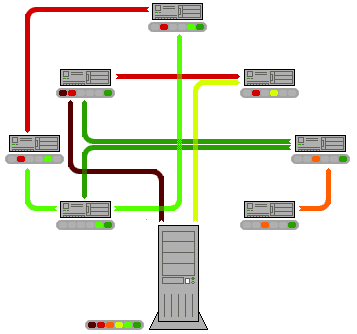
\includegraphics[width=80mm]{imagenes/animation/bittorrent-animation-3}
  \end{figure}
\end{frame}

% Animacion 4
\begin{frame} \frametitle{El protocolo BitTorrent}
\vspace{-2mm}
  \begin{figure}[H]
    \centering
    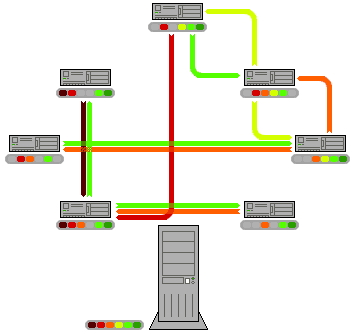
\includegraphics[width=80mm]{imagenes/animation/bittorrent-animation-4}
  \end{figure}
\end{frame}

% Animacion 5
\begin{frame} \frametitle{El protocolo BitTorrent}
\vspace{-2mm}
  \begin{figure}[H]
    \centering
    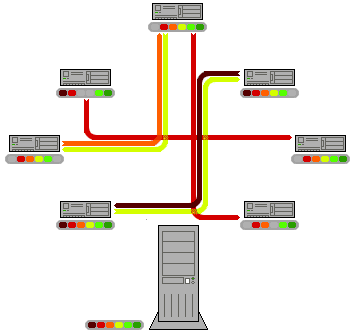
\includegraphics[width=80mm]{imagenes/animation/bittorrent-animation-5}
  \end{figure}
o\end{frame}

% Animacion 6
\begin{frame} \frametitle{El protocolo BitTorrent}
\vspace{-2mm}
  \begin{figure}[H]
    \centering
    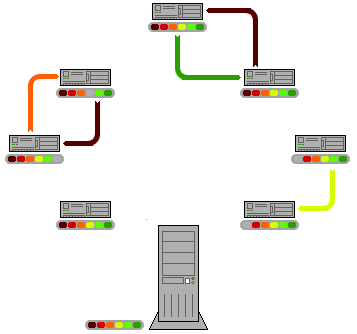
\includegraphics[width=80mm]{imagenes/animation/bittorrent-animation-6}
  \end{figure}
\end{frame}

% Animacion 7
\begin{frame} \frametitle{El protocolo BitTorrent}
\vspace{-2mm}
  \begin{figure}[H]
    \centering
    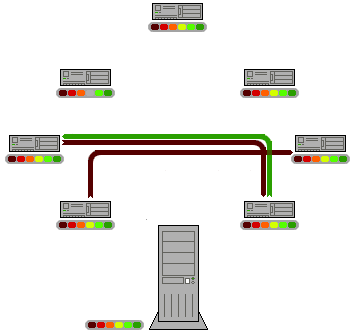
\includegraphics[width=80mm]{imagenes/animation/bittorrent-animation-7}
  \end{figure}
\end{frame}

% Animacion 8
\begin{frame} \frametitle{El protocolo BitTorrent}
\vspace{-2mm}
  \begin{figure}[H]
    \centering
    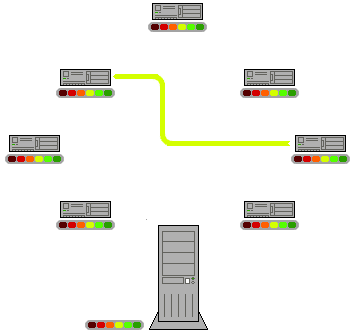
\includegraphics[width=80mm]{imagenes/animation/bittorrent-animation-8}
  \end{figure}
\end{frame}

% Animacion 9
\begin{frame} \frametitle{El protocolo BitTorrent}
\vspace{-2mm}
  \begin{figure}[H]
    \centering
    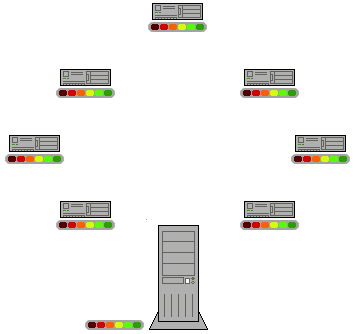
\includegraphics[width=80mm]{imagenes/animation/bittorrent-animation-9}
  \end{figure}
\end{frame}

\subsection{Otros mecanismos de funcionamiento}

\begin{frame}\frametitle{Otros mecanismos de funcionamiento}
  \begin{itemize}
  \item Pipelining y mini-chunks.
  \item Prioridad Estricta a completar chunks.
  \item Endgame Mode.
  \item Anti-Snubbing.
  \item Primera Pieza Aleatoria.
  \item Solo subida.
  \item UDP Tracker.
  \end{itemize}
\end{frame}

\section{Wireshark}
\subsection{Conexi�n con Tracker}

\begin{frame}\frametitle{Conexi�n con Tracker}
  \begin{figure}[H]
  \centering
  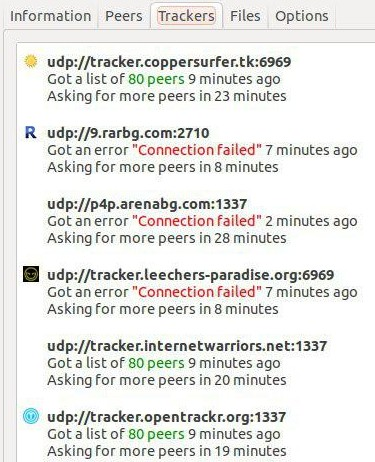
\includegraphics[width=45mm]{imagenes/tracker_transmission}
  \caption{Captura de Transmision: Lista de los trackers a los que nos conectamos para descargar el archivo.}
\end{figure}
\end{frame}

\begin{frame}\frametitle{Conexi�n con Tracker}
\begin{figure}[H]
  \centering
  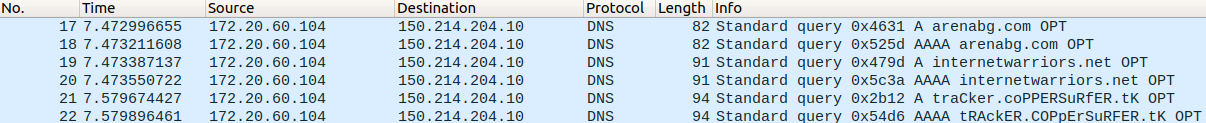
\includegraphics[width=115mm]{imagenes/trackers}
  \caption{Captura de Wireshark: Conexi�n con trackers.}
\end{figure}

\begin{figure}[H]
  \centering
  
\includegraphics[width=115mm]{imagenes/arenabg}
  \caption{Captura de Wireshark: Intercambio de mensajes para la conexi�n al tracker ``arenabg''. Estos mensajes se hacen con protocolo DNS, que usa UDP internamente.}
\end{figure}
\end{frame}

\begin{frame}\frametitle{Conexi�n con Tracker}
  \vspace{-3mm}
\begin{figure}[H]
  \centering
  \subfigure{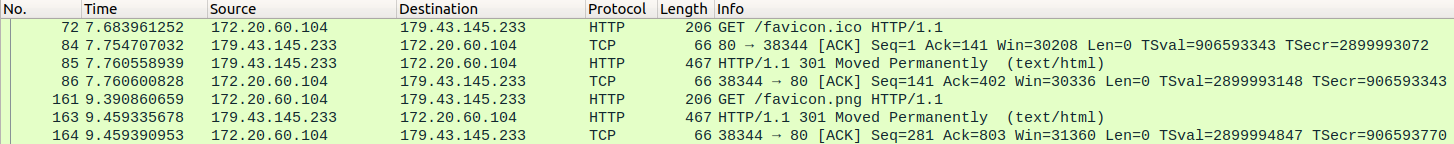
\includegraphics[width=115mm]{imagenes/http}}
  \subfigure{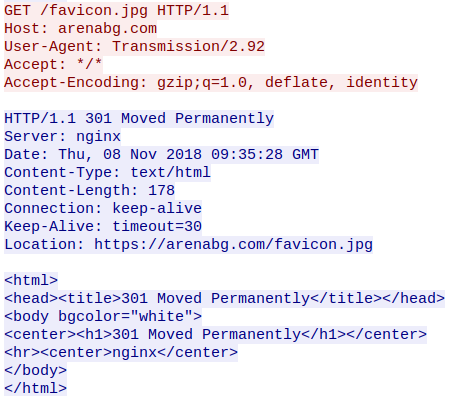
\includegraphics[width=54mm]{imagenes/tcp-http-arenabg}}
  \caption{Captura de Wireshark: Usando el protocolo HTTP, nos comunicamos con el tracker.}
\end{figure}
\end{frame}

\begin{frame}\frametitle{Conexi�n con Tracker}
  \vspace{-5mm}
\begin{figure}[H]
  \centering
  \subfigure{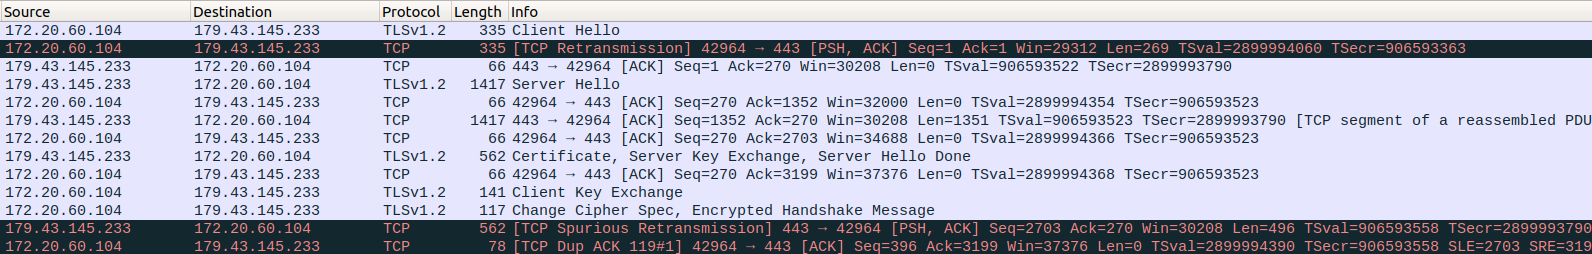
\includegraphics[width=110mm]{imagenes/tcp-tracker-conversation}}
  \subfigure{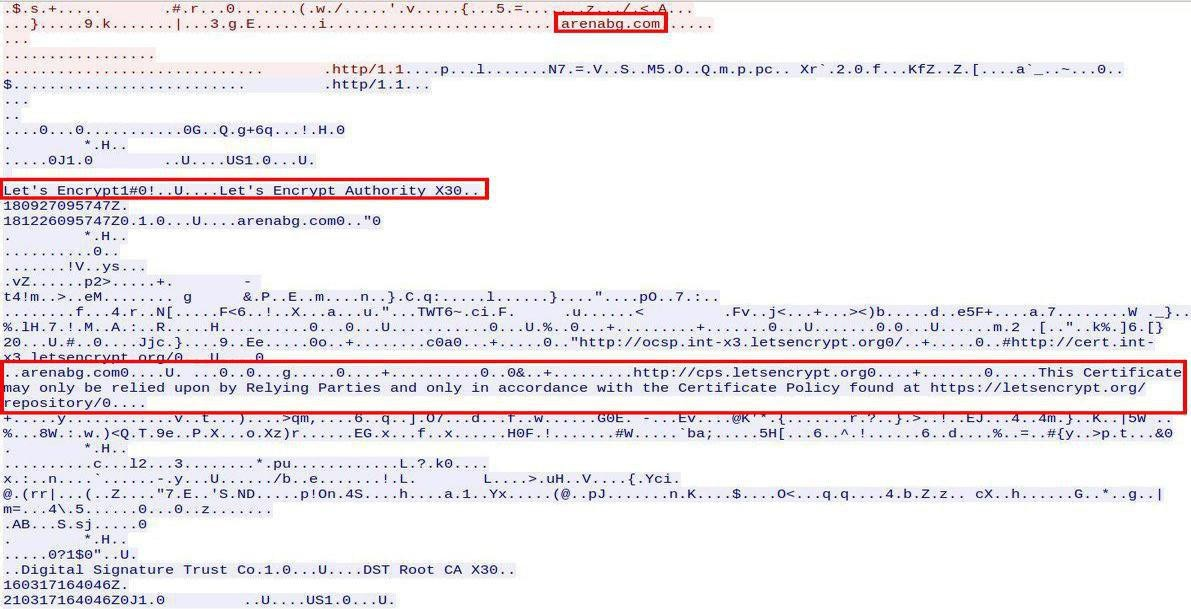
\includegraphics[width=107mm]{imagenes/trama_arenabg_resaltado}}
\end{figure}
\end{frame}

\subsection{Conexi�n con Peers}

\begin{frame}\frametitle{Conexi�n con Peers}
\begin{figure}[H]
  \centering
  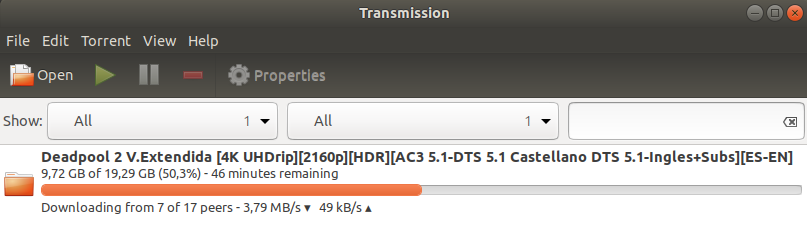
\includegraphics[width=115mm]{imagenes/transmission-deadpool}
  \caption{Captura de Transmision.}
\end{figure}
\end{frame}

\begin{frame}\frametitle{Conexi�n con Peers}
\begin{figure}[H]
  \centering
  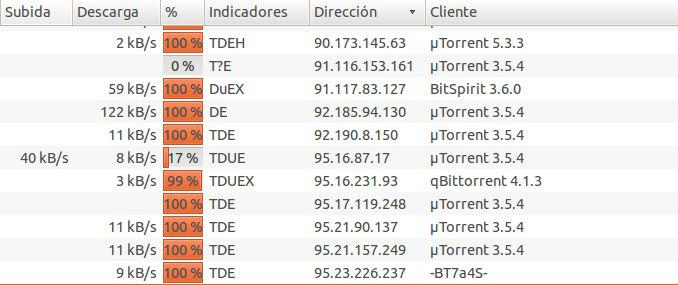
\includegraphics[width=115mm]{imagenes/peers}
  \caption{Captura de Transmision: Los peer con los que nos estamos comunicando, nuestros ``vecinos''.}
\end{figure}
\end{frame}

\begin{frame}\frametitle{Conexi�n con Peers}
\begin{figure}[H]
  \centering
  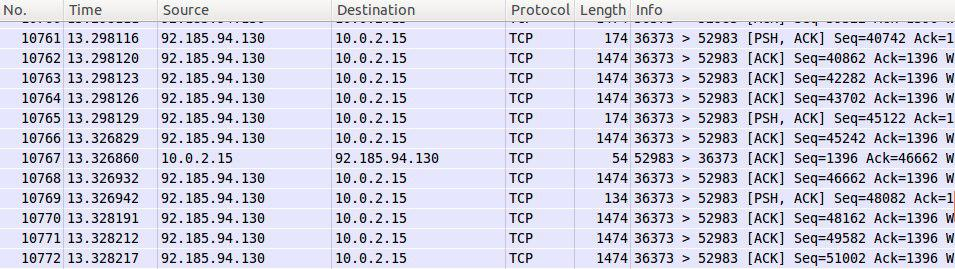
\includegraphics[width=115mm]{imagenes/TCP_wireshark}
  \caption{Captura Wireshark.}
\end{figure}
\end{frame}

\begin{frame}\frametitle{Conexi�n con Peers}
\begin{figure}[H]
  \centering
  \caption{Conversaci�n entre peers (TCP Flow)}
  \subfigure{
\includegraphics[width=52mm]{imagenes/trama_rojo}}
  \hfill
  \subfigure{
\includegraphics[width=52mm]{imagenes/trama_azul}}
\end{figure}
\end{frame}

\begin{frame}\frametitle{Conexi�n con Peers}
\begin{figure}[H]
  \centering
  \subfigure{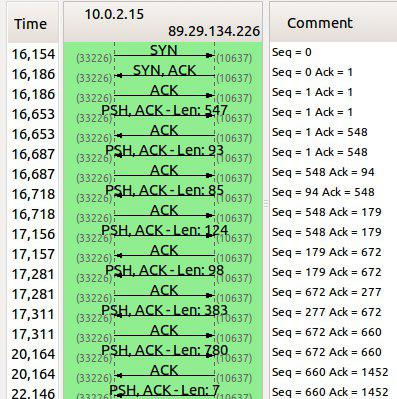
\includegraphics[width=50mm]{imagenes/statistic_flow}}
  \hfill
  \subfigure{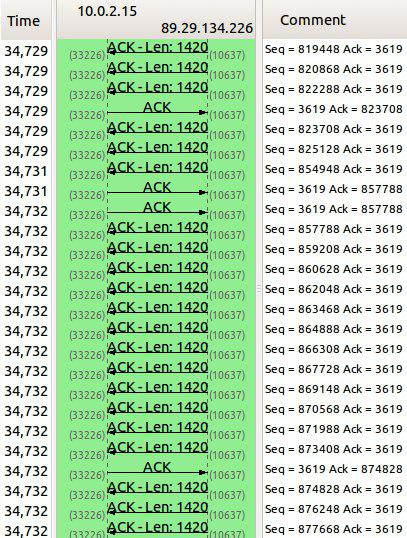
\includegraphics[width=45mm]{imagenes/statistic_flow1}}
  \caption{Flow Graph.}
\end{figure}
\end{frame}

\section{Referencias}
\begin{frame}\frametitle{Referencias}
  \begin{itemize}
\item \href{https://en.wikipedia.org/wiki/BitTorrent}{https://en.wikipedia.org/wiki/BitTorrent}
\item Jim Kurose, Keith Ross, \href{https://www.bau.edu.jo/UserPortal/UserProfile/PostsAttach/10617_1870_1.pdf}{``Computer Networking: A Top-Down Approach''}, Pearson, 2013, pp. 144-151.
\item Bram Cohen, \href{http://bittorrent.org/bittorrentecon.pdf}{``Incentives Build Robustness in BitTorrent''}, 2003.
\item \href{https://wiki.wireshark.org/BitTorrent}{https://wiki.wireshark.org/BitTorrent}
\item \href{https://en.wikipedia.org/wiki/UDP_tracker}{https://en.wikipedia.org/wiki/UDP\_tracker}
\end{itemize}  
\end{frame}

\end{document}